%% Timelines: LifeSpans

\addcontentsline{toc}{section}{TImeline of the course: philosophers, painters, poets and other thinkers}

%% Puts new lifespan to the diagram
%% Arguments:
%% Arg1: Start year
%% Arg2: End year
%% Arg3: Description
%% Arg4: Color
%% Optional argument: node parameters (e.g., anchor)
\newcommand{\putLifeSpan}[5][]{%
%% Starting position for the lifespan
\pgfmathsetlengthmacro{\startPos}{(((#2>\constStartYear) ? #2 : \constStartYear) - \constStartYear)*\constMminYear}
%% End position of the lifespan
\pgfmathsetlengthmacro{\endPos}{(((#3<\constStopYear) ? #3 : \constStopYear) - \constStartYear)*\constMminYear}
%% Center position of the lifespan - to put the label there
\pgfmathsetlengthmacro{\centerPos}{(\endPos + \startPos)/2}
\draw[rounded corners=1mm,fill=#5] (\startPos, 0) rectangle (\endPos, \constLifeSpanHeight);
\node[#1] at (\centerPos, \constLifeSpanHeight + 2mm) {#4 (#2--#3)};
}

%% Draws vertical tics for the timeline
%% Arg1: Year
\newcommand{\drawVertTics}[1]{%
%% X pos
\pgfmathsetlengthmacro{\pos}{(#1 - \constStartYear)*\constMminYear}
\draw[ultra thin,densely dotted] (\pos, 1cm) -- (\pos, .9\textheight);
\node at (\pos, 0) {#1};
}

%% Philosophers
\colorlet{lifespancolorph}{MidnightBlue}
%% Painters
\colorlet{lifespancolorpa}{ForestGreen}
%% Writers and poets
\colorlet{lifespancolorwr}{Fuchsia}
%% All others (default)
\colorlet{lifespancolor}{Gray}


%% Updates shift
\newcommand{\updateshift}{\pgfmathsetlengthmacro{\myshift}{\myshift + .85cm}}

\newcommand{\colsign}[1]{\colorbox{#1}{\hspace*{1cm}}}
\newsavebox{\thinkers}
\savebox{\thinkers}{\Large\itshape\parbox{7cm}{%
\begin{itemize}
\item[\colsign{lifespancolorph}] Philosophers
\item[\colsign{lifespancolorpa}] Painters
\item[\colsign{lifespancolorwr}] Poets and Prose Writers
\item[\colsign{lifespancolor}] Others
\end{itemize}}}

\noindent\hspace*{.25cm}\copyrightbox[b]{%
\begin{tikzpicture}[x=1mm,y=1mm]
\pgfmathsetlengthmacro{\constLifeSpanHeight}{2mm}
\pgfmathsetmacro{\constStartYear}{1700}%
\pgfmathsetmacro{\constStopYear}{1840}%
\pgfmathsetlengthmacro{\myshift}{1cm}%
%% Scale: points in one year
\pgfmathsetlengthmacro{\constMminYear}{.9\textwidth/(\constStopYear-\constStartYear)}
%% Grid
\foreach \i in {1700,1720,...,1840} {
\drawVertTics{\i}
}
%% Lifespans
\begin{scope}[yshift=\myshift]
\putLifeSpan{1711}{1776}{David Hume}{lifespancolorph}
\putLifeSpan{1780}{1867}{Jean Ingres}{lifespancolorpa}
\end{scope}
\updateshift
\begin{scope}[yshift=\myshift]
\putLifeSpan{1712}{1778}{Jean-Jacques Rousseau}{lifespancolorph}
\putLifeSpan{1798}{1863}{Eugène Delacroix}{lifespancolorpa}
\end{scope}
\updateshift
\begin{scope}[yshift=\myshift]
\putLifeSpan{1724}{1804}{Immanuel Kant}{lifespancolorph}
\putLifeSpan{1806}{1873}{John Stuart Mill}{lifespancolorph}
\end{scope}
\updateshift
\begin{scope}[yshift=\myshift]
\putLifeSpan[anchor=west]{1632}{1704}{John Locke}{lifespancolorph}
\putLifeSpan{1748}{1832}{Jeremy Bentham}{lifespancolorph}
\end{scope}
\updateshift
\begin{scope}[yshift=\myshift]
\putLifeSpan{1770}{1831}{Georg Wilhelm Friedrich Hegel}{lifespancolorph}
\end{scope}
\updateshift
\begin{scope}[yshift=\myshift]
\putLifeSpan{1770}{1850}{William Wordsworth}{lifespancolorwr}
\end{scope}
\updateshift
\begin{scope}[yshift=\myshift]
\putLifeSpan{1772}{1834}{Samuel Taylor Coleridge}{lifespancolorwr}
\end{scope}
\updateshift
\begin{scope}[yshift=\myshift]
\putLifeSpan{1802}{1892}{Constantin Guys}{lifespancolor}
\end{scope}
\updateshift
\begin{scope}[yshift=\myshift]
\putLifeSpan{1809}{1882}{Charles Darwin}{lifespancolor}
\end{scope}
\updateshift
\begin{scope}[yshift=\myshift]
\putLifeSpan{1803}{1882}{Ralph Emerson}{lifespancolorph}
\end{scope}
\updateshift
\begin{scope}[yshift=\myshift]
\putLifeSpan[font=\small]{1815}{1898}{Otto von Bismarck}{lifespancolor}
\end{scope}
\updateshift
\begin{scope}[yshift=\myshift]
\end{scope}
\updateshift
\begin{scope}[yshift=\myshift]
\end{scope}
\updateshift
\begin{scope}[yshift=\myshift]
\end{scope}
\updateshift
\begin{scope}[yshift=\myshift]
\end{scope}
\updateshift
\begin{scope}[yshift=\myshift]
\end{scope}
\updateshift
\begin{scope}[yshift=\myshift]
\end{scope}
\node at (55,100) { \usebox{\thinkers} };
\node[font=\Huge\scshape\bfseries,fill=blue!20,rounded corners] at (80, 140) {1632 -- 1984};
\end{tikzpicture}}{\centerline{\myLicense}}
\newpage

\hspace*{.25cm}\copyrightbox[b]{%
\begin{tikzpicture}[x=1mm,y=1mm]
\pgfmathsetlengthmacro{\constLifeSpanHeight}{2mm}
\pgfmathsetmacro{\constStartYear}{1840}%
\pgfmathsetmacro{\constStopYear}{1984}%
\pgfmathsetlengthmacro{\myshift}{1cm}%
%% Scale: points in one year
\pgfmathsetlengthmacro{\constMminYear}{.9\textwidth/(\constStopYear-\constStartYear)}
%% Grid
\foreach \i in {1840,1860,...,1980} {
\drawVertTics{\i}
}
%% Lifespans
\begin{scope}[yshift=\myshift]
\putLifeSpan{1780}{1867}{Jean Ingres}{lifespancolorpa}
\putLifeSpan{1872}{1970}{Bertrand Russell}{lifespancolorph}
\end{scope}
\updateshift
\begin{scope}[yshift=\myshift]
\putLifeSpan{1864}{1901}{Toulouse-Lautrec}{lifespancolorpa}
\end{scope}
\updateshift
\begin{scope}[yshift=\myshift]
\putLifeSpan{1806}{1873}{John Stuart Mill}{lifespancolorph}
\putLifeSpan{1881}{1973}{Pablo Picasso}{lifespancolorpa}
\end{scope}
\updateshift
\begin{scope}[yshift=\myshift]
\putLifeSpan{1834}{1917}{Edgar Degas}{lifespancolorpa}
\end{scope}
\updateshift
\begin{scope}[yshift=\myshift]
\putLifeSpan{1832}{1883}{Édouard Manet}{lifespancolorpa}
\putLifeSpan{1887}{1927}{Juan Gris}{lifespancolorpa}
\end{scope}
\updateshift
\begin{scope}[yshift=\myshift]
\putLifeSpan{1856}{1939}{Sigmund Freud}{lifespancolor}
\end{scope}
\updateshift
\begin{scope}[yshift=\myshift]
\putLifeSpan{1839}{1906}{Paul Cézanne}{lifespancolorpa}
\putLifeSpan{1912}{1956}{Jackson Pollock}{lifespancolorpa}
\end{scope}
\updateshift
\begin{scope}[yshift=\myshift]
\putLifeSpan{1802}{1892}{Constantin Guys}{lifespancolor}
\putLifeSpan{1895}{1973}{Max Horkheimer}{lifespancolorph}
\end{scope}
\updateshift
\begin{scope}[yshift=\myshift]
\putLifeSpan{1809}{1882}{Charles Darwin}{lifespancolor}
\putLifeSpan{1887}{1968}{Marcel Duchamp}{lifespancolorpa}
\end{scope}
\updateshift
\begin{scope}[yshift=\myshift]
\putLifeSpan{1803}{1882}{Ralph Emerson}{lifespancolorph}
\putLifeSpan{1889}{1951}{Ludwig Wittgenstein}{lifespancolorph}
\end{scope}
\updateshift
\begin{scope}[yshift=\myshift]
\putLifeSpan{1815}{1898}{Otto von Bismarck}{lifespancolor}
\putLifeSpan{1903}{1969}{Theodor W. Adorno}{lifespancolorph}
\end{scope}
\updateshift
\begin{scope}[yshift=\myshift]
\putLifeSpan{1818}{1883}{Karl Heinrich Marx}{lifespancolorph}
\putLifeSpan{1926}{1984}{Michel Foucault}{lifespancolorph}
\end{scope}
\updateshift
\begin{scope}[yshift=\myshift]
\putLifeSpan{1821}{1880}{Gustave Flaubert}{lifespancolorwr}
\putLifeSpan{1882}{1941}{Virginia Woolf}{lifespancolorwr}
\end{scope}
\updateshift
\begin{scope}[yshift=\myshift]
\putLifeSpan{1819}{1877}{Gustave Courbet}{lifespancolorpa}
\end{scope}
\updateshift
\begin{scope}[yshift=\myshift]
\putLifeSpan{1821}{1867}{Baudelaire}{lifespancolorwr}
\putLifeSpan{1873}{1958}{George Edward Moore}{lifespancolorph}
\end{scope}
\updateshift
\begin{scope}[yshift=\myshift]
\putLifeSpan{1830}{1903}{Camille Pissarro}{lifespancolorpa}
\end{scope}
\updateshift
\begin{scope}[yshift=\myshift]
\putLifeSpan{1844}{1900}{Friedrich Wilhelm Nietzsche}{lifespancolorph}
\end{scope}
\end{tikzpicture}}{\centerline{\myLicense}}


